\documentclass[aps,pre,reprint,twocolumn,showkeys,nofootinbib,superscriptaddress,floatfix]{revtex4-2}

% ---------------------------------------------------------------
% PACKAGES
% ---------------------------------------------------------------
\usepackage{amsmath,amssymb}
\usepackage{graphicx}
\usepackage{booktabs}
\usepackage{lmodern}
\usepackage[expansion=false]{microtype}
\usepackage{xcolor}
\usepackage{enumitem}
\usepackage{algpseudocode}
\renewcommand{\algorithmicrequire}{\textbf{Input:}}
\renewcommand{\algorithmicensure}{\textbf{Output:}}

\usepackage[colorlinks=true,citecolor=green!60!black,linkcolor=blue!70!black,urlcolor=blue!70!black]{hyperref}

% ---------------------------------------------------------------
% DOCUMENT
% ---------------------------------------------------------------
\begin{document}

\title{ADCD: Correction-First Symbolic Regression with Formal Identifiability Guarantees}

\author{Muhammad Afif Erdita}
\email{maeapip10@gmail.com}
\affiliation{Independent Researcher, Indonesia}

\date{\today}

\begin{abstract}
    We present \textbf{ADCD} (Asymptotic Dictionary Correction Discovery), a
    deterministic symbolic regression framework that discovers corrections to
    known physical laws with formal identifiability guarantees.
    Standard symbolic regression engines are designed to recover complete
    equations from scratch, representing a fundamentally broader objective
    than correction discovery.
    We show that this difference has measurable consequences: at zero noise, an unconstrained SR baseline (PySR) structurally recovers the
    correct functional form in $10$--$50\%$ of independent runs
    ($n = 20$ seeds) despite achieving comparable or superior training fit,
    while ADCD structurally recovers it in $90$--$100\%$ of runs.
    This gap reflects a structural tradeoff (since fit quality and structural
    identifiability are independent evaluation dimensions) rather than a
    limitation of either approach within its intended scope.
    ADCD enforces identifiability through three core mechanisms:
    a bounded dictionary of algebraically regularized primitives that vanish
    at the classical limit by construction (with physically motivated exceptions explicitly flagged), eliminating catastrophic cancellation in the evaluation of $D(u)$ as $u \to 0$;
    a tiered filter cascade integrating dimensional relaxation, asymptotic boundary probes, and coarse/fine parameter fitting;
    and a post-fitting four-step epistemic validation protocol that
    explicitly withholds or qualifies structural claims when data are insufficient.
    Evaluated on three canonical physics scenarios across $165$ unique
    data instances (scenario $\times$ seed $\times$ noise level),
    ADCD demonstrates consistent structural recovery under both noiseless
    and noisy conditions ($1\%$--$30\%$ Gaussian noise). Crucially, ADCD explicitly differentiates between structural search success and formal epistemic certification: across all 165 runs, ADCD formally certified 112 runs as \texttt{IDENTIFIABLE}, explicitly qualified 53 runs as \texttt{DETECTED\_UNRESOLVED} due to SNR-limited ambiguity, and assigned 0 false positives to the null hypothesis.
\end{abstract}

\keywords{symbolic regression, correction discovery, structural identifiability, dimensional analysis, Bayesian model selection}

\maketitle

% ---------------------------------------------------------------
\section{Introduction}
% ---------------------------------------------------------------

Physical laws often follow a correction-first structure: a known classical baseline is extended by a term that vanishes at the classical limit~\cite{einstein1905,debye1923,callen1985,vanderwaals1873,michelson1887}. Modern symbolic regression (SR) engines (e.g., genetic programming~\cite{koza1994}, Eureqa~\cite{schmidt2009}, AI Feynman~\cite{udrescu2020}, PySR~\cite{cranmer2023}) are designed for unconstrained equation recovery, which is a fundamentally broader objective than correction discovery. When applied to the narrower correction task, three structural challenges arise: catastrophic cancellation as $\Delta \to 0$ corrupts gradient signals even in \texttt{float64}; stochastic multi-objective search~\cite{bongard2007,deb2002} over unconstrained expression spaces is computationally hard~\cite{virgolin2022} and precludes deterministic reproducibility; and the absence of explicit identifiability reporting means a single ``best'' answer is returned regardless of whether the data genuinely support a structural claim~\cite{lacava2021}.

Even in the idealized noiseless setting, unconstrained SR can converge to expressions that are numerically indistinguishable from the true law on the training domain but structurally distinct. This is not a software deficiency but a well-understood consequence of the parsimony principle: on narrow observation domains, multiple function classes achieve comparable fit, and complexity-penalized selection has no algebraic mechanism to prefer the physically generating structure over a simpler numerical approximation. We term this the \emph{parsimony--identifiability tradeoff}.

We present ADCD, a correction-first framework that assumes the classical
baseline is known and searches only for the residual correction.
Algebraically regularized primitives eliminate catastrophic cancellation
by construction.
Candidates are assembled by deterministic grammar enumeration and evaluated through a tiered filter cascade integrating dimensional relaxation, asymptotic boundary probes, and coarse/fine parameter fitting before formal epistemic certification.
Identifiability is explicitly reported via a post-fitting four-step
validation protocol: ADCD withholds structural claims when
evidence is ambiguous.

We validate ADCD across three canonical physics domains:
relativity (Time Dilation, $v \le 0.3c$), electrostatics (Screened Coulomb, $r \le 4.0$), and thermodynamics (Entropy Expansion, $dV/V_i \le 3.0$).
Under zero noise ($n = 20$ independent seeds), ADCD recovers the generating functional class in $90$--$100\%$ of runs across all three scenarios; PySR recovers it in $10$--$50\%$ depending on the scenario.
Extrapolation errors (median held-out NMSE $\le 10^{-7}$ for ADCD) and noise-sweep experiments ($1\%$--$30\%$ noise, $n = 5$ seeds, $105$ runs) further characterize the structural robustness of the two paradigms.

% ---------------------------------------------------------------
\section{Related Work}
\label{sec:related}
% ---------------------------------------------------------------

Symbolic regression has evolved along two distinct trajectories. \textbf{Unconstrained SR engines} (Eureqa~\cite{schmidt2009}, PySR~\cite{cranmer2023}, AI Feynman~\cite{udrescu2020,udrescu2020b}, $\Phi$-SO~\cite{tenachi2023}, symbolic regression with neural networks~\cite{cranmer2020}) perform open-ended equation discovery without prior knowledge of the underlying physical law. \textbf{Physics-informed discovery} frameworks incorporate constraints: SINDy~\cite{brunton2016,rudy2017,rackauckas2020} searches linear combinations of predefined library terms for dynamical systems; PINNs~\cite{raissi2019,karniadakis2021} embed differential equation residuals into neural loss functions; $\Phi$-SO~\cite{tenachi2023} enforces dimensional consistency via reinforcement learning; and grammar-guided SR~\cite{petersen2021,li2019,cornelio2023} restricts search spaces using domain grammars. Model selection in SR typically relies on the Pareto frontier of loss versus complexity, or information criteria (AIC~\cite{akaike1974}, BIC~\cite{schwarz1978}, Kass--Raftery thresholds~\cite{kass1995}).

ADCD occupies a distinct point in this space: it restricts search exclusively to corrections of known physical laws, enforces asymptotic boundary conditions algebraically by construction rather than through loss penalties or grammar rules, and implements an explicit epistemic validation protocol that reports WITHHELD when identifiability cannot be established.

We emphasize that the tools compared here address conceptually different problems. General SR engines target unconstrained equation discovery across arbitrary functional forms, representing a broader and fundamentally harder problem than correction discovery. ADCD deliberately restricts its scope to corrections of known baselines, trading generality for stronger identifiability guarantees within this narrower domain. The comparison presented in Section~\ref{sec:experiments} is therefore not evaluative (which approach is ``better'') but characterizing: it examines how different design choices (parsimony-driven selection versus identifiability-driven selection) manifest in structural recovery behavior when applied to the same correction tasks.

Table~\ref{tab:paradigms} summarizes the key design distinctions between ADCD and related frameworks.

\begin{table*}[t]
\caption{Conceptual comparison of scientific equation discovery frameworks.
``Hard algebraic'' means the constraint is imposed as an exact symbolic identity,
not a soft penalty or regularization term.}
\label{tab:paradigms}
\begin{ruledtabular}
\begin{tabular}{lllll}
Framework & Search space & Classical-limit constraint & Identifiability reporting & Primary objective \\
\hline
Standard SR~\cite{schmidt2009,cranmer2023} & Free expression tree & None & None (best fit returned) & Open-ended discovery \\
SINDy~\cite{brunton2016}        & Polynomial library & None & Parsimony threshold & Dynamical sparse identification \\
PINNs~\cite{raissi2019}         & Neural network & Soft loss penalty & None & PDE forward/inverse solving \\
AI Feynman~\cite{udrescu2020}   & Free tree + symmetry & Dimensional/separability tests & None & Physics equation cracking \\
AI Descartes~\cite{cornelio2023}& Axiom theory + data & Logical axioms & Formal derivability & Theory-consistent regression \\
\textbf{ADCD (ours)}            & Regularized primitive dict. & \textbf{Hard algebraic (exact)} & \textbf{Formal $\Delta$BIC + WITHHELD} & \textbf{Certified physical corrections} \\
\end{tabular}
\end{ruledtabular}
\end{table*}

% ---------------------------------------------------------------
\section{Methods}
\label{sec:methods}

\begin{figure*}[t]
\centering
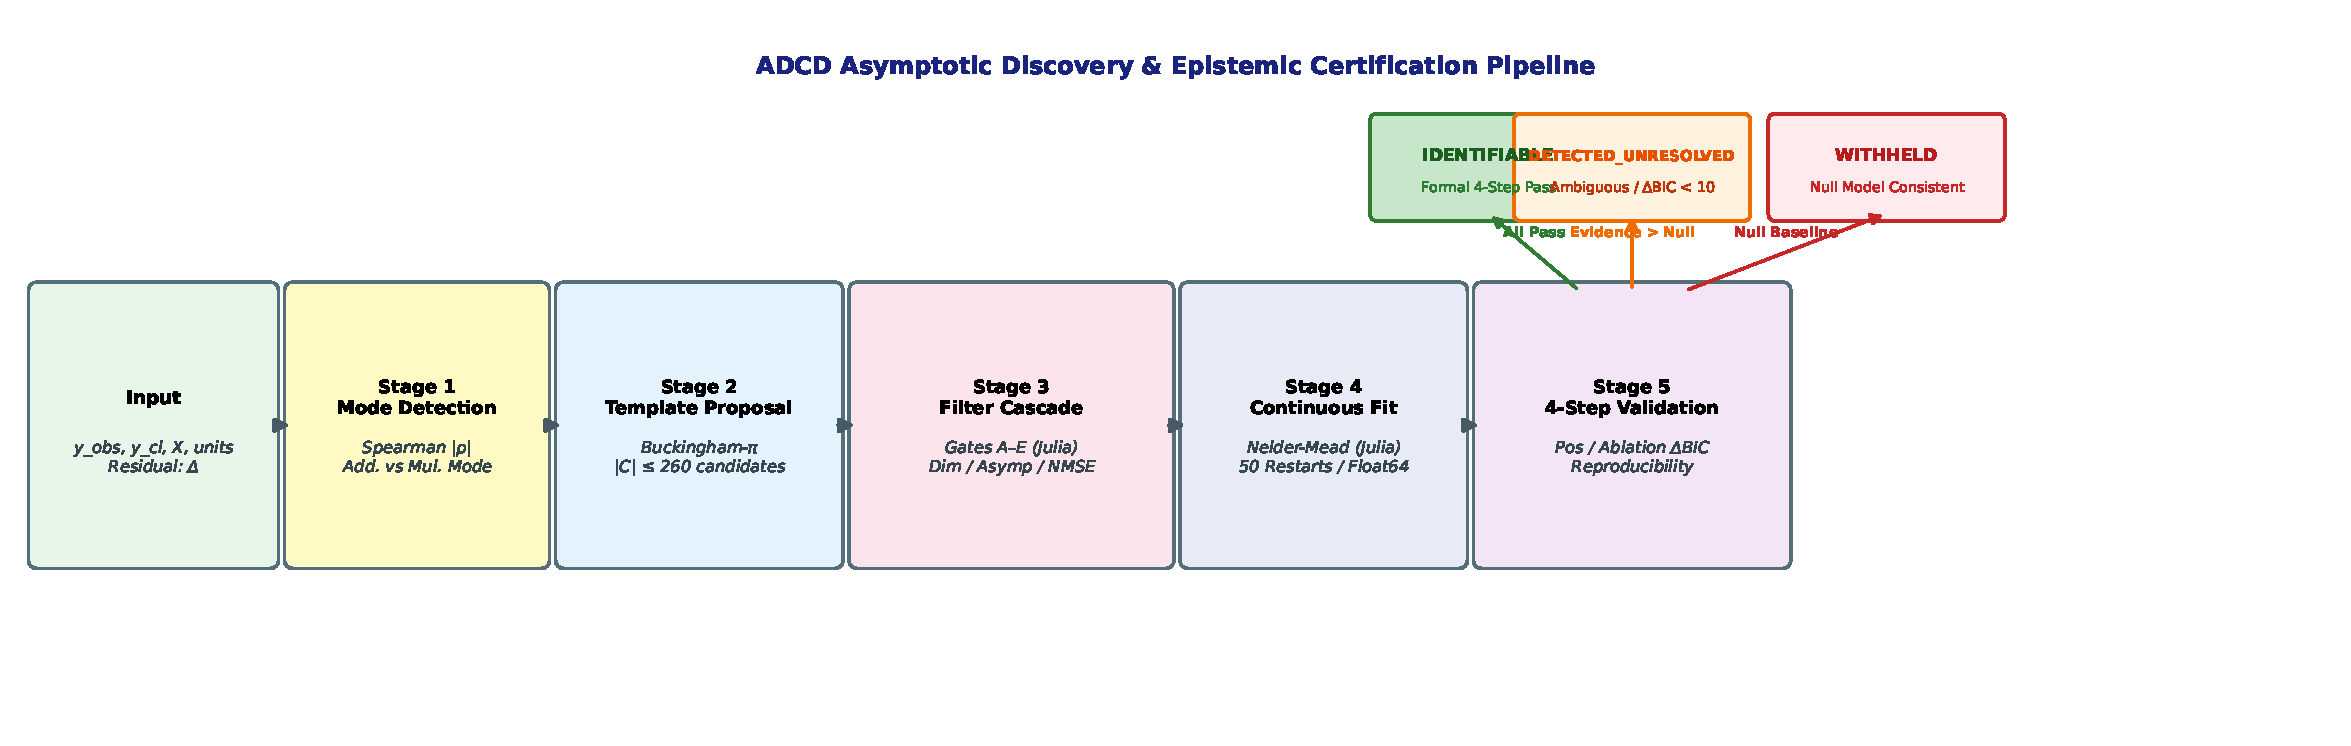
\includegraphics[width=\textwidth]{fig4_pipeline.pdf}
\caption{The ADCD discovery and certification pipeline. Raw inputs $(y_\mathrm{obs}, y_\mathrm{cl}, \mathbf{X}, \mathcal{U})$ enter Stage~1 (dynamic mode selection via Spearman $|\rho|$). Stage~2 generates dimensionless arguments via Buckingham-$\pi$ with degree pruning and applies 6 structural templates. Stage~3 screens candidates through a tiered filter cascade (dimensional relaxation, numerical asymptotic boundary probe, coarse/fine Nelder--Mead parameter optimization, and Gate~E EBIC null test). Stage~5 applies the 4-step post-fitting epistemic validation protocol (budget disclosure, positive control, ablation margin $\Delta\mathrm{BIC}_\mathrm{ablation} \ge 10.0$, and computational reproducibility), yielding a 3-tier verdict (\texttt{IDENTIFIABLE}, \texttt{DETECTED\_UNRESOLVED}, or \texttt{WITHHELD}).}
\label{fig:pipeline}
\end{figure*}

\subsection{Problem formulation}

Let $y_\mathrm{obs}$ be the observed target and $y_\mathrm{cl}$ the known
classical prediction.
Define the correction residual:
\begin{equation}
  \Delta =
  \begin{cases}
    y_\mathrm{obs}/y_\mathrm{cl} - 1 & \text{(multiplicative)} \\
    y_\mathrm{obs} - y_\mathrm{cl}   & \text{(additive)}
  \end{cases}
\end{equation}
ADCD dynamically selects between the two formulations via a Spearman rank-correlation test
(Algorithm~\ref{alg:mode} in Appendix~\ref{app:algorithms}):
the multiplicative form is selected when the residual magnitude is less correlated
with the classical prediction magnitude than the additive residual is.
The intuition is that a multiplicative correction $\Delta_\mathrm{mul} = y_\mathrm{obs}/y_\mathrm{cl} - 1$
is scale-normalized and should be \emph{independent} of $|y_\mathrm{cl}|$; strong correlation
of $|\Delta_\mathrm{add}|$ with $|y_\mathrm{cl}|$ therefore indicates that the additive
residual has not been normalized out, confirming multiplicative mode.
If $|y_\mathrm{cl}|$ has zero variance or fewer than 5 observations are available,
the algorithm defaults to the additive formulation.
ADCD then searches for $\hat{\Delta}(\mathbf{x};\boldsymbol{\theta})$, where
$\mathbf{x}$ is the vector of physical inputs, $\boldsymbol{\theta}$ are
continuous free parameters, and $\hat{\Delta} \to 0$ as the relevant
dimensionless parameter $u \to 0$.

\subsection{Regularized primitive dictionary}
\label{sec:primitives}

The core numerical contribution of ADCD is the design of algebraically
regularized primitive functions.
Except for specialized forms with physically motivated divergent boundaries, each asymptotically regularized primitive $D(u)$ satisfies $\lim_{u\to 0} D(u) = 0$ as an exact algebraic
identity, not a numerical approximation.
While primitives are designed to vanish exactly by construction, the pre-fitting asymptotic boundary verification employs a robust three-tier protocol. It prioritizes exact symbolic limit evaluation (via SymPy), but autonomously falls back to Laurent series expansions and numerical boundary probes ($u \approx 10^{\pm 6}$) to ensure computational stability when evaluating complex transcendental argument compositions.
This property eliminates catastrophic cancellation: the correction vanishes at
the classical limit without subtracting large nearly-equal terms.

While the full production registry (implemented in \texttt{PrimitiveRegistry.jl}) contains 11 primitives spanning relativistic kinematics, screening, saturation, phase transitions, oscillatory resonance, and MOND phenomenology, Table~\ref{tab:primitives} lists the 5 principal regularized primitives evaluated in the benchmark suite of this paper.
The practical consequence is demonstrated for \texttt{D\_lor}: in
\texttt{float32}, the naive form $(1-u)^{-1/2} - 1$ collapses to exactly 0.0
at $u = 10^{-8}$; in \texttt{float64}, precision degrades progressively
(11\% relative error at $u = 10^{-15}$; total collapse at $u = 10^{-16}$).
The regularized form $u\,/\,[\sqrt{1-u}(\sqrt{1-u}+1)]$ preserves full
precision at all scales, returning $5.0 \times 10^{-17}$ at $u = 10^{-16}$
where the naive form returns 0.0 (in numerical evaluation, a floating-point safety bound $u \le 1 - 10^{-9}$ is enforced to prevent division-by-zero at the singular horizon).

\begin{table}[t]
\caption{The five principal algebraically regularized primitives evaluated in this study. Each satisfies
$\lim_{u\to0} D(u) = 0$ as an exact algebraic identity.}
\label{tab:primitives}
\begin{ruledtabular}
\begin{tabular}{lll}
Name & Regularized form $D(u)$ & Domain \\
\hline
\texttt{D\_lor}       & $u\,/\,[\sqrt{1-u}(\sqrt{1-u}+1)]$ & $u \in [0,1)$ \\
\texttt{D\_rat}       & $u\,/\,(1+u^2)$                      & $u \in \mathbb{R}$ \\
\texttt{D\_exp}       & $1 - e^{-|u|}$                        & $u \in \mathbb{R}$ \\
\texttt{D\_log}       & $\ln(1+|u|)$                         & $u \in \mathbb{R}$ \\
\texttt{D\_sqrt\_inv} & $\sqrt{|u|}\,/\,(1+\sqrt{|u|})$    & $u \in \mathbb{R}$ \\
\end{tabular}
\end{ruledtabular}
\end{table}

The 6 additional registered primitives in the general registry include power-law anomalous scaling (\texttt{D\_pow}: $\sqrt{|u|}(1-e^{-|u|})$), Langevin saturation (\texttt{D\_sat}: $\tanh(u)$), symmetric transition (\texttt{D\_tanh\_sq}: $\tanh(u^2)$), oscillatory interference (\texttt{D\_osc}: $1 - \cos(u)$), asymmetric nested anomaly (\texttt{D\_nested\_mond}: $e^{-\sqrt{|u|}}(1-e^{-\sqrt{|u|}})$), and the McGaugh Radial Acceleration Relation quotient form (\texttt{D\_rar}: $e^{-\sqrt{u}}/(1-e^{-\sqrt{u}})$). The \texttt{D\_rar} primitive is explicitly flagged as \texttt{divergent\_safe} with limit $D(u\to 0)\to \infty$ and $D(\infty)\to 0$, and is conditionally restricted to deep-MOND regimes.

\subsection{Grammar enumeration and template patterns}
\label{sec:grammar}

Rather than unconstrained recursive grammar growth, ADCD constructs candidates through a bounded combinatorial templating engine (implemented in \texttt{CorrectionProposer.jl}). Candidate expressions are generated by mapping regularized primitives $D_i(u)$ and dimensionless arguments $u_{ij}$ across six explicit structural templates:
\begin{enumerate}[noitemsep,leftmargin=*]
  \item \textbf{Singleton:} $\hat{\Delta} = \theta_0 \cdot D(u)$
  \item \textbf{Additive composite:} $\hat{\Delta} = \theta_1 D_a(u) + \theta_2 D_b(u)$
  \item \textbf{Multiplicative composite:} $\hat{\Delta} = \theta_1 D_a(u) \cdot \bigl(1 + \theta_2 D_b(u)\bigr)$
  \item \textbf{Nested composition:} $\hat{\Delta} = \theta_0 \cdot D_a\bigl(D_b(u)\bigr)$
  \item \textbf{Bilateral interaction:} $\hat{\Delta} = \theta_0 \cdot D_a(u_1) \cdot D_b(u_2)$ for distinct dimensionless arguments $u_1 \neq u_2$
  \item \textbf{Ratio correction:} $\hat{\Delta} = \theta_0 \cdot \frac{D(\sqrt{u})}{1 + D(\sqrt{u})}$
\end{enumerate}

The dimensionless arguments $u_{ij}$ are generated via Buckingham-$\pi$ permutation of input variables, classical constants, and scale parameters. To prevent combinatorial explosion, the generator enforces strict heuristic pruning: polynomial degrees are capped ($\mathrm{degree} \le 2$), and pure constant ratios ($c_1/c_2$) are discarded.
The search space is bounded by an AST complexity cap (depth $\le 12$, nodes $\le 50$), yielding a compact, exhaustively enumerable pool of candidate ASTs (e.g., $|\mathcal{C}| = 35$ in guided mode, $|\mathcal{C}| = 140$--$260$ in blind mode across our benchmark scenarios), fully proposed in milliseconds.

All candidate structures maintain free parameters $\boldsymbol{\theta}$ throughout the filtering and fitting pipeline (\emph{theta-intact}). Filtering gates never strip or default $\boldsymbol{\theta}$ parameters to arbitrary constants, as stripping alters functional curvature and invalidates physical consistency checks.

\subsection{Tiered filter cascade and parameter optimization}
\label{sec:cascade}

Before exhaustive continuous optimization and model selection, each candidate AST passes through a tiered filter cascade (implemented in \texttt{FilterCascade.jl}):
\begin{enumerate}[noitemsep,leftmargin=*]
  \item \textbf{Gate A (Dimensional consistency with theta-relaxation):} Verifies that the candidate has the physical dimensions of the residual $\Delta$. Crucially, arguments of transcendental functions containing free parameters $\theta$ are dimensionally relaxed, as continuous optimization assigns inverse units to $\theta$ to render the composite argument dimensionless.
  \item \textbf{Gate B (Numerical asymptotic boundary probe):} Evaluates the candidate at the asymptotic boundary $u = 10^{-12}$ with nominal parameters $\boldsymbol{\theta} = \mathbf{1}$. Candidates failing $|D(u)| < 10^{-4}$ are rejected without expensive optimization.
  \item \textbf{Gate C (Coarse parameter pre-fit):} Executes a lightweight continuous fit via Nelder--Mead ($n_\mathrm{restarts} = 3$). Candidates with coarse loss $\mathrm{NMSE} > 1.0$ are pruned early.
  \item \textbf{Gate D (Fine parameter fit):} Surviving candidates undergo full continuous parameter optimization using \texttt{Optim.jl} Nelder--Mead ($n_\mathrm{restarts} = 50$) in \texttt{float64} precision across five initialization scales ($10^{-6}$ to $10^6$) with quadrant sign permutations and log-uniform exponent sampling to robustly escape non-convex local minima.
  \item \textbf{Gate E (Identifiability and EBIC certification vs null model):} Evaluates the candidate against the classical null model ($\Delta = 0$).
\end{enumerate}

Loss is normalized mean squared error:
\begin{equation}
  \mathrm{NMSE} = \frac{\frac{1}{N} \sum_i (\hat{\Delta}_i - \Delta_i)^2}{\max\bigl(\frac{1}{N-1} \sum_i (\Delta_i - \bar{\Delta})^2,\, \epsilon\bigr)}
\end{equation}
To ensure numerical stability in regimes with extreme scaling, ADCD dynamically monitors the observation range: if $\max(|y|) / \min(|y|) > 10^4$, the loss target shifts from residual space $\Delta$ to full observation space $y_\mathrm{obs}$.

Surviving candidates are ranked by the Extended Bayesian Information Criterion (EBIC)~\cite{chen2008}, which incorporates a complexity penalty for the size of the candidate dictionary $|\mathcal{C}|$:
\begin{equation}
  \mathrm{EBIC} = k \ln N - 2\ln\hat{L} + 2 \ln |\mathcal{C}|
\end{equation}
where $k$ is the number of free continuous parameters, $N$ is the effective sample size, and $\hat{L}$ is the maximized Gaussian likelihood.
The candidate is certified at Gate~E if it outperforms the classical null baseline by $\Delta\mathrm{BIC}_\mathrm{gate} = \mathrm{BIC}_\mathrm{null} - \mathrm{EBIC}_\mathrm{corr} \ge 10.0$.

In addition to identifying the Rank-1 candidate, ADCD implements Bayesian Model Averaging (BMA) via \texttt{bayesian\_ranker.py}, computing posterior model weights, structural class probabilities, and posterior entropy to quantify structural ambiguity when competing functional forms achieve comparable fit.

\subsection{Post-fitting four-step epistemic validation}
\label{sec:validation}

Rather than returning the single best-fitting expression unconditionally,
ADCD applies a four-step post-fitting validation protocol (implemented in \texttt{run\_adcd\_v3\_validation\_blind.py}) to assign candidates to one of three epistemic tiers:

\begin{enumerate}[noitemsep,leftmargin=*]
  \item \textbf{Gate V.1 (Search budget disclosure):} Total candidates generated, evaluated, and pruned are logged with all operator budgets.
  \item \textbf{Gate V.2 (Positive control):} The optimizer is evaluated on a restricted candidate space containing only the isolated target primitive family, verifying that numerical optimization reliably converges to low loss ($\mathrm{NMSE} \le 0.1$) when given the true functional class alone.
  \item \textbf{Gate V.3 (Ablation control):} An ablated search is performed with the winning primitive class removed from the dictionary. The true model must outperform the best available alternative by a decisive Bayesian margin ($\Delta\mathrm{BIC}_\mathrm{ablation} = \mathrm{EBIC}_\mathrm{ablated} - \mathrm{EBIC}_\mathrm{candidate} \ge 10.0$).
  \item \textbf{Gate V.4 (Computational reproducibility):} Three independent runs with identical inputs produce byte-exact identical numerical and symbolic results via deterministic cryptographic seeding of the optimizer's \texttt{MersenneTwister}. This serves as a software sanity check, not a formal epistemic proof.
\end{enumerate}

ADCD classifies discovery results into three formal epistemic outcome tiers:
\begin{itemize}[noitemsep,leftmargin=*]
  \item \textbf{\texttt{IDENTIFIABLE}:} The candidate passes all four validation gates with decisive evidence ($\Delta\mathrm{BIC}_\mathrm{ablation} \ge 10.0$) and verified positive control.
  \item \textbf{\texttt{DETECTED\_UNRESOLVED}:} Strong evidence of a physical anomaly is confirmed against the classical null model ($\Delta\mathrm{BIC}_\mathrm{gate} \ge 10.0$), but the candidate fails either Gate V.2 (Positive control) or Gate V.3 (Ablation control margin $< 10.0$). This outcome explicitly informs the researcher that real physics beyond the baseline exists, but the observation domain or SNR is insufficient to unequivocally isolate the true functional form from competing alternatives.
  \item \textbf{\texttt{WITHHELD}:} The data are consistent with pure Gaussian noise around the classical baseline ($\Delta\mathrm{BIC}_\mathrm{gate} < 10.0$), non-convergence, or reproducibility failure, confirming that the classical baseline alone is sufficient.
\end{itemize}

\begin{table*}[t]
\hrule height 0.8pt
\vspace{3pt}
\noindent\textbf{Algorithm 1:} \textit{ADCD Epistemic Discovery and Certification Protocol}
\label{alg:adcd}
\vspace{2pt}
\hrule height 0.4pt
\vspace{4pt}
\noindent\textbf{Input:} Observed array $y_\mathrm{obs}$, classical baseline $y_\mathrm{cl}$, feature matrix $\mathbf{X} = \{x_j\}$, SI unit declarations $\mathcal{U}$, observation window $\Omega$, evidence threshold $\Delta\mathrm{BIC}^* = 10.0$.\\
\textbf{Output:} Epistemic verdict $v \in \{\texttt{IDENTIFIABLE}, \texttt{DETECTED\_UNRESOLVED}, \texttt{WITHHELD}\}$, certified expression $\hat{\Delta}$, parameter estimates $\boldsymbol{\theta}^*$, Bayes factors, machine-readable audit trail.
\vspace{3pt}
\hrule height 0.4pt
\vspace{4pt}
\begin{algorithmic}[1]
\Function{EpistemicDiscovery}{$y_\mathrm{obs}, y_\mathrm{cl}, \mathbf{X}, \mathcal{U}, \Omega, \Delta\mathrm{BIC}^*$}
    \State \textbf{// Stage 1: Mode Detection (Algorithm~\ref{alg:mode})}
    \State $\text{mode}, \kappa \leftarrow \textsc{DetectMode}(y_\mathrm{obs}, y_\mathrm{cl})$
    \State $\Delta \leftarrow (y_\mathrm{obs}/y_\mathrm{cl} - 1)$ \textbf{if} $\text{mode} = \texttt{multiplicative}$ \textbf{else} $(y_\mathrm{obs} - y_\mathrm{cl})$
    
    \vspace{0.2em}
    \State \textbf{// Stage 2: Dimensionless Grammar Proposal}
    \State $\{u_{ij}\} \leftarrow \textsc{BuckinghamPi}(\mathbf{X}, \mathcal{U})$ \Comment{dimensionless argument pool with pruning}
    \State $\mathcal{C} \leftarrow \textsc{ApplyTemplates}(\mathcal{D}, \{u_{ij}\})$ \Comment{6 structural patterns; $|\mathcal{C}| \le 260$}
    
    \vspace{0.2em}
    \State \textbf{// Stage 3: Tiered Filter Cascade and Optimization (FilterCascade.jl)}
    \State $\mathcal{C}_\mathrm{valid} \leftarrow \emptyset$
    \For{\textbf{each} candidate $c \in \mathcal{C}$}
        \If{$\textsc{IsDimensionlessRelaxed}(c, \mathcal{U})$ \textbf{and} $\textsc{AsymptoticProbe}(c, 10^{-12}) < 10^{-4}$}
            \State $\boldsymbol{\theta}_c^\mathrm{coarse} \leftarrow \textsc{NelderMead}(c, \Delta, \text{restarts}=3)$
            \If{$\mathrm{NMSE}(\boldsymbol{\theta}_c^\mathrm{coarse}) \le 1.0$}
                \State $\boldsymbol{\theta}_c^* \leftarrow \textsc{NelderMead}(c, \Delta, \text{restarts}=50)$ \Comment{fine fit}
                \State $\mathrm{EBIC}_c \leftarrow k_c \ln N - 2\ln\hat{L}_c + 2\ln|\mathcal{C}|$
                \State $\mathcal{C}_\mathrm{valid} \leftarrow \mathcal{C}_\mathrm{valid} \cup \{(c, \boldsymbol{\theta}_c^*, \mathrm{EBIC}_c)\}$
            \EndIf
        \EndIf
    \EndFor
    
    \vspace{0.2em}
    \State \textbf{// Stage 4: Model Ranking and Gate E Null Test}
    \If{$\mathcal{C}_\mathrm{valid} = \emptyset$}
        \State \Return $\langle\texttt{WITHHELD},\; \text{None},\; \text{None},\; 0.0\rangle$
    \EndIf
    \State $\hat{c}, \boldsymbol{\theta}^*, \mathrm{EBIC}^*, \mathrm{NMSE}^* \leftarrow \arg\min_{(c,\boldsymbol{\theta},\mathrm{EBIC}) \in \mathcal{C}_\mathrm{valid}} \mathrm{EBIC}$
    \State $\Delta\mathrm{BIC}_\mathrm{gate} \leftarrow \mathrm{BIC}_\mathrm{null} - \mathrm{EBIC}^*$
    \If{$\Delta\mathrm{BIC}_\mathrm{gate} < \Delta\mathrm{BIC}^*$ \textbf{or} $\mathrm{NMSE}^* > \mathrm{NMSE}_\mathrm{max}$}
        \State \Return $\langle\texttt{WITHHELD},\; \hat{c},\; \boldsymbol{\theta}^*,\; \Delta\mathrm{BIC}_\mathrm{gate}\rangle$
    \EndIf
    
    \vspace{0.2em}
    \State \textbf{// Stage 5: Four-Step Post-Fitting Epistemic Validation}
    \State $\text{pass}_\mathrm{pos} \leftarrow \textsc{PositiveControl}(\hat{c}, \Omega_0)$
    \State $\Delta\mathrm{BIC}_\mathrm{ablation} \leftarrow \textsc{AblationControl}(\hat{c}, \mathcal{D} \setminus \{\text{class}(\hat{c})\})$
    \State $\text{pass}_\mathrm{det} \leftarrow \textsc{ReproducibilityCheck}(\hat{c})$
    
    \If{$\text{pass}_\mathrm{det}$ \textbf{and} $\text{pass}_\mathrm{pos}$ \textbf{and} $\Delta\mathrm{BIC}_\mathrm{ablation} \ge \Delta\mathrm{BIC}^*$}
        \State \Return $\langle\texttt{IDENTIFIABLE},\; \hat{c},\; \boldsymbol{\theta}^*,\; \Delta\mathrm{BIC}_\mathrm{ablation}\rangle$
    \Else
        \State \Return $\langle\texttt{DETECTED\_UNRESOLVED},\; \hat{c},\; \boldsymbol{\theta}^*,\; \Delta\mathrm{BIC}_\mathrm{ablation}\rangle$
    \EndIf
\EndFunction
\end{algorithmic}
\vspace{3pt}
\hrule height 0.8pt
\end{table*}


% ---------------------------------------------------------------
\section{Experiments}
\label{sec:experiments}
% ---------------------------------------------------------------

\subsection{Experimental setup}

We evaluate ADCD on three canonical synthetic physics scenarios, summarized
in Table~\ref{tab:scenarios}.
The observation windows are chosen to reflect varying degrees of physical
identifiability: from strict low-signal regimes of early historical
experiments (e.g., $v \le 0.3c$ for Time Dilation, where the relativistic
correction is $\le 5\%$ of the classical prediction) to broader macroscopic
domains required for thermodynamic identifiability (e.g., $dV/V_i \le 3.0$
for Entropy Expansion, where the logarithmic form becomes structurally
distinguishable from polynomial alternatives).
To maintain IEEE 754 floating-point stability during nonlinear optimization, synthetic raw variables (e.g., mass, charge, distance) are generated in normalized macroscopic $\mathcal{O}(1)$ units. However, the dimensionless arguments driving the structural anomaly (such as $v/c$ or $r/\lambda$) strictly mirror the geometric regimes of historical laboratory observations.

We select PySR~\cite{cranmer2023} as our primary baseline, not because it
is expected to solve the same problem as ADCD, but because it represents
the state-of-the-art in general-purpose symbolic regression and provides
a well-characterized reference point for understanding how structural
recovery behavior differs between constrained correction discovery and
unconstrained equation search.
PySR is run with its default configuration and standard operator set
($+, -, \times, /, \exp, \log, \sqrt{\cdot}, \sin, \cos$).
For both ADCD and the PySR baseline, recovery is evaluated on the
\textbf{single top-ranked expression} returned by each algorithm's default
model selection logic: the Pareto-optimal candidate with lowest BIC score
for ADCD, and PySR's highest-scoring expression under its default parsimony
criterion (accessed via \texttt{model.sympy()}).

Two ADCD variants are evaluated: \emph{guided} (with domain taxonomy prior restricting primitives) and \emph{blind} (full dictionary, no domain hints), to isolate the contribution of taxonomy information. Evaluation uses two complementary experimental regimes:
\begin{enumerate}[noitemsep,leftmargin=*]
  \item \textbf{Zero-noise baseline} ($n = 20$ seeds per scenario, $60$ runs total): isolates structural recovery capability independent of noise.
  \item \textbf{Noise-level sweep} ($7$ levels from $1\%$ to $30\%$, $n = 5$ seeds, $105$ runs total): observational noise is injected multiplicatively ($y_\mathrm{obs} = y_\mathrm{true}(1 + \epsilon)$, $\epsilon \sim \mathcal{N}(0, \sigma^2)$) for multiplicative corrections, characterizing how relative measurement noise modulates structural recovery.
\end{enumerate}

Structural recovery is evaluated via functional class recovery: an expression
is counted as \emph{recovered} if its functional class matches the
generating equation's class and its fitted parameters yield physically
consistent extrapolation behavior
($\mathrm{NMSE}_\mathrm{extrap} < 2.0$, $|\theta_i| < 10^6$).
This metric measures \textbf{search capability} (whether the correct
functional class is identified) and is distinct from the
\textbf{epistemic certification} provided by the post-fitting four-step
validation protocol (Section~\ref{sec:validation}).
A run may satisfy the structural match criterion while still receiving a
WITHHELD verdict if $\Delta\mathrm{BIC} \le 10$; in that case, the
correct structure was found but the data are insufficient to formally
certify the claim.
The threshold $\mathrm{NMSE}_\mathrm{extrap} < 2.0$ acts as a coarse filter
to reject catastrophic pole singularities and floating-point overflow
(e.g., failed extrapolations, such as PySR on Screened Coulomb, routinely shoot to $\mathrm{NMSE}_\mathrm{extrap} > 1000$ outside the training domain);
precise median extrapolation errors (e.g., $\le 10^{-7}$ for ADCD at zero noise)
are reported separately in Section~\ref{sec:extrap}.
The threshold reflects an empirically observed bimodal gap: across all
165 unique data instances ($60$ noiseless $+$ $105$ noise-sweep, evaluated
across $495$ total algorithm passes), no run falls between
$\mathrm{NMSE}_\mathrm{extrap} = 1.69$ and $3.37$.

\begin{table}[t]
\caption{The three validated scenarios with their domains, observation windows, and target primitives.
Full quantitative results (BIC, $\Delta$BIC, verdicts) are in Table~\ref{tab:results}.}
\label{tab:scenarios}
\begin{ruledtabular}
\footnotesize
\begin{tabular}{llll}
Scenario & Domain & Window & Target Primitive \\
\hline
Time Dilation     & Relativity     & $v \le 0.3c$          & \texttt{D\_lor} \\
Screened Coulomb  & Electrostatics & $r \le 4.0$           & \texttt{D\_exp} \\
Entropy Expansion & Thermodynamics & $dV/V_i \le 3.0$     & \texttt{D\_log} \\
\end{tabular}
\end{ruledtabular}
\end{table}

\subsection{Structural recovery at zero noise}
\label{sec:zeronoise}

Table~\ref{tab:zeronoise} presents the headline experiment: structural recovery rates under zero-noise conditions ($n = 20$ independent seeds per scenario). This setting isolates the effect of search strategy and inductive bias from noise-related confounds.

\begin{table}[t]
\caption{Structural recovery rates at zero noise ($n = 20$ seeds). Wilson 95\% confidence intervals in brackets. ADCD guided and blind variants produce identical verdicts across all 60 runs.}
\label{tab:zeronoise}
\begin{ruledtabular}
\footnotesize
\begin{tabular}{lccc}
Scenario & ADCD (guided/blind) & PySR (default) & CI overlap \\
\hline
Time Dilation     & $100\%$ [$84$--$100\%$] & $10\%$ [$3$--$30\%$]  & None \\
Screened Coulomb  & $100\%$ [$84$--$100\%$] & $50\%$ [$30$--$70\%$] & None \\
Entropy Expansion & $90\%$ [$70$--$97\%$]   & $25\%$ [$11$--$47\%$] & None \\
\end{tabular}
\end{ruledtabular}
\end{table}

ADCD recovers the generating functional form in $90$--$100\%$ of runs,
while PySR recovers it in $10$--$50\%$ depending on the scenario.
These tools address conceptually different objectives: PySR, optimized for
fit quality under parsimony pressure, converges to compact expressions that
achieve low training error but may differ structurally from the generating
functional form.
ADCD, optimized for structural identifiability under asymptotic constraints,
recovers the correct functional form at the cost of a narrower search scope.

Three characteristic behavioral patterns illustrate the parsimony--identifiability tradeoff:

\textbf{Trigonometric basis selection.} PySR's genetic search explores trigonometric bases ($\sin$, $\cos$) as compact approximators for non-trigonometric target functions. For example, $\sin(v)$ provides a low-complexity approximation to the Lorentz factor on narrow velocity domains, representing a rational search strategy under parsimony pressure.

\textbf{High-precision fit with structural divergence.} In several zero-noise runs, PySR achieves training NMSE comparable to or better than ADCD while producing a structurally distinct expression. This directly illustrates that numerical fit quality and structural recovery are independent evaluation axes.

\textbf{Domain-width sensitivity.} PySR's recovery rate varies substantially across scenarios ($10\%$ for Time Dilation vs.\ $50\%$ for Screened Coulomb), correlating with the curvature of the generating function within the observation window. This is consistent with the parsimony--identifiability tradeoff: when the generating function's distinctive curvature is more pronounced, parsimony-driven selection more frequently converges to the correct structure.

\subsection{Noise-level sweep}

Having established that structural recovery differences exist independent of
noise (\S\ref{sec:zeronoise}), we examine how observation noise modulates
this behavior.
Table~\ref{tab:noisesweep} summarizes recovery rates across seven noise
levels ($n = 5$ seeds each, $105$~runs total).
ADCD's recovery on Time Dilation is robust across the entire noise range
($100\%$ at all seven levels); Screened Coulomb and Entropy Expansion show
degradation at high noise, consistent with weaker signal-to-noise on the
correction residual.
PySR's recovery is more variable, with high variance across noise levels
for Screened Coulomb at $n = 5$, reflecting the sensitivity of
parsimony-driven search to random seed at small sample size.
Overall, ADCD maintains a structural recovery advantage across the noise
range, with the advantage most pronounced at high noise levels ($\ge 0.20$)
where PySR's recovery approaches zero in most scenarios.

\begin{table*}[t]
\caption{Structural recovery rate (\%) vs.\ noise level ($n = 5$ seeds per
point, $105$~runs total). Full Wilson 95\% confidence interval detail is provided in Appendix Table~\ref{tab:noisesweep_ci}.}
\label{tab:noisesweep}
\begin{ruledtabular}
\begin{tabular}{lcccccc}
& \multicolumn{2}{c}{Time Dilation} & \multicolumn{2}{c}{Screened Coulomb} & \multicolumn{2}{c}{Entropy Expansion} \\
Noise ($\sigma$) & ADCD & PySR & ADCD & PySR & ADCD & PySR \\
\hline
0.01 & 100 &  60 &  80 &   0 & 100 & 20 \\
0.02 & 100 &  60 &  80 &  60 & 100 &  0 \\
0.05 & 100 &  60 & 100 &  40 & 100 &  0 \\
0.10 & 100 &  40 &  80 &  20 &  80 &  0 \\
0.15 & 100 &  20 &  80 &  60 &  80 &  0 \\
0.20 & 100 &  20 &  60 &   0 &  60 &  0 \\
0.30 & 100 &   0 &  20 &   0 &  40 &  0 \\
\end{tabular}
\end{ruledtabular}
\end{table*}

\begin{figure*}[t]
  \centering
  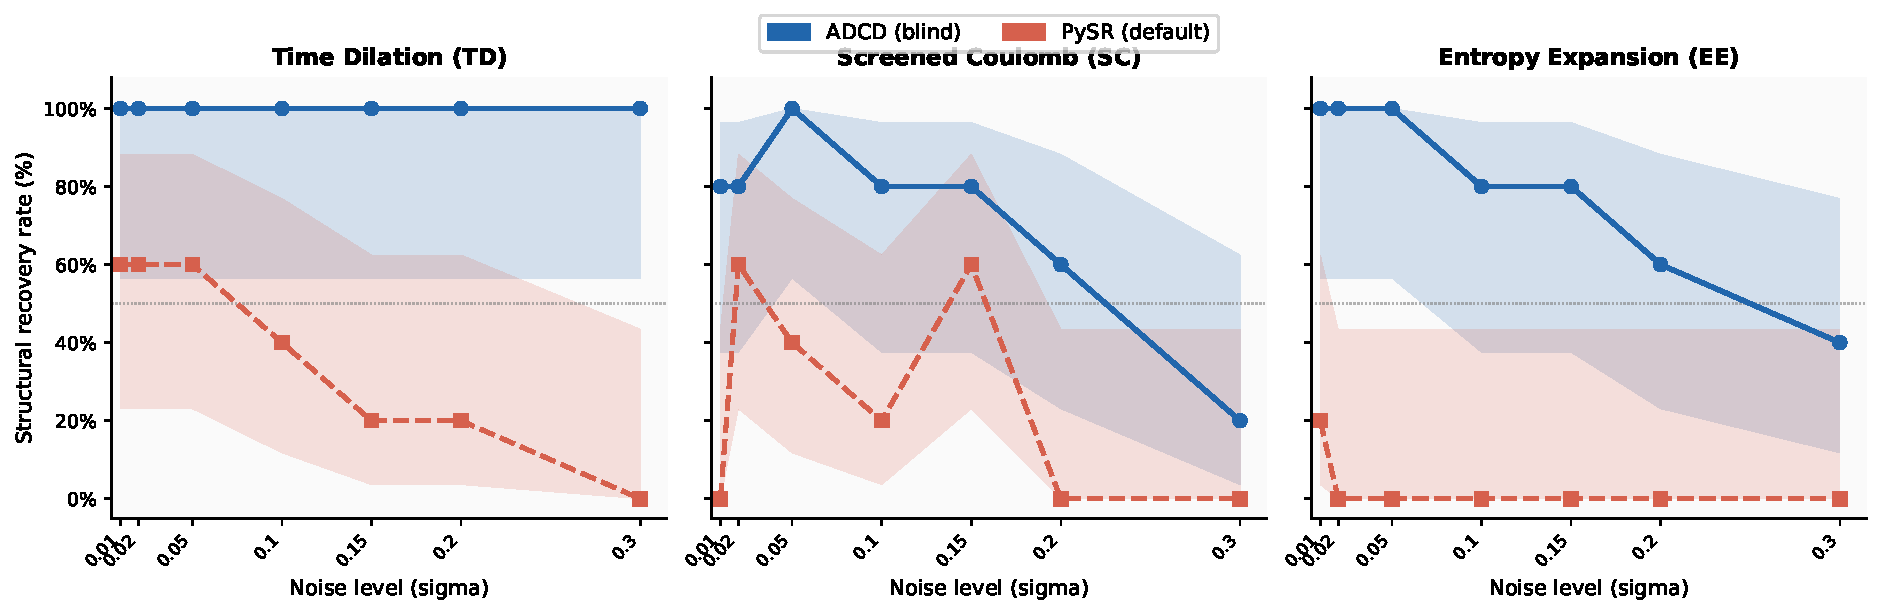
\includegraphics[width=\textwidth]{fig3_noisesweep.pdf}
  \caption{%
    Structural recovery rate (\%) vs.\ noise level $\sigma$ for the three scenarios ($n=5$ seeds per point;
    shaded bands: Wilson 95\% CI).
    ADCD (blue, solid) consistently maintains higher recovery across all noise levels.
    PySR (red, dashed) recovery approaches zero for Screened Coulomb and Entropy Expansion
    at $\sigma \ge 0.20$, reflecting the parsimony--identifiability tradeoff under noisy conditions.
    Wilson 95\% CI detail is tabulated in Appendix Table~\ref{tab:noisesweep_ci}.
  }
  \label{fig:noisesweep}
\end{figure*}

\subsection{Extrapolation behavior}
\label{sec:extrap}

We evaluate out-of-domain generalization to examine whether asymptotic regularization (a design feature of ADCD but not of general SR) translates to improved extrapolation consistency.
Held-out extrapolation evaluation is conducted strictly on non-overlapping extended domains: $v \in (0.3c, 0.8c]$ for Time Dilation, $r \in (4.0, 8.0]$ for Screened Coulomb, and $dV/V_i \in (3.0, 6.0]$ for Entropy Expansion.
ADCD's expressions, constrained to vanish at the classical limit by construction, maintain physical consistency outside the training domain: across the zero-noise experiment ($n = 20$ seeds), median extrapolation NMSE is below $10^{-7}$ for all three scenarios.
PySR's expressions, not designed with extrapolation constraints, exhibit variable behavior depending on the functional form selected. The most pronounced illustration is in the Screened Coulomb zero-noise experiment: PySR's worst-case extrapolation NMSE reaches $1530.5$ across $20$ seeds (median: $0.054$), reflecting runs where the selected expression diverges outside the training domain.
We explicitly acknowledge that this extrapolation metric is inherently biased towards ADCD by design. It highlights the mathematical reality of standard SR when unconstrained by boundary conditions, rather than indicating a defect in PySR itself. PySR is a general unconstrained exploratory engine, whereas ADCD is heavily specialized to force algebraic primitives to vanish at the classical limit.

\subsection{Ablation: taxonomy contribution}
\label{sec:ablation}

Across all $165$~unique data instances ($60$ noiseless $+$ $105$ noise-sweep), the formal
epistemic verdict (tier) is identical between ADCD-guided and ADCD-blind
in $100\%$ of cases.
Domain taxonomy reduces the candidate search space for each primitive
class while preserving the identifiability boundary across both configurations.
In our benchmark suite, the guided variant evaluates a single hand-fed dimensionless ratio ($|\mathcal{C}| = 35$), whereas the blind variant auto-derives multi-ratio permutations via Buckingham-$\pi$ ($|\mathcal{C}| = 140$--$260$) over the identical core primitive pool.
This demonstrates that ADCD's automated dimensionless argument generation reliably discovers the true physical scale arguments without human guidance, though comprehensive evaluation across the broader 11-primitive dictionary represents an important area for future large-scale replication.

\subsection{Recovered structures and identifiability verdicts}
\label{sec:results}

\begin{figure*}[t]
  \centering
  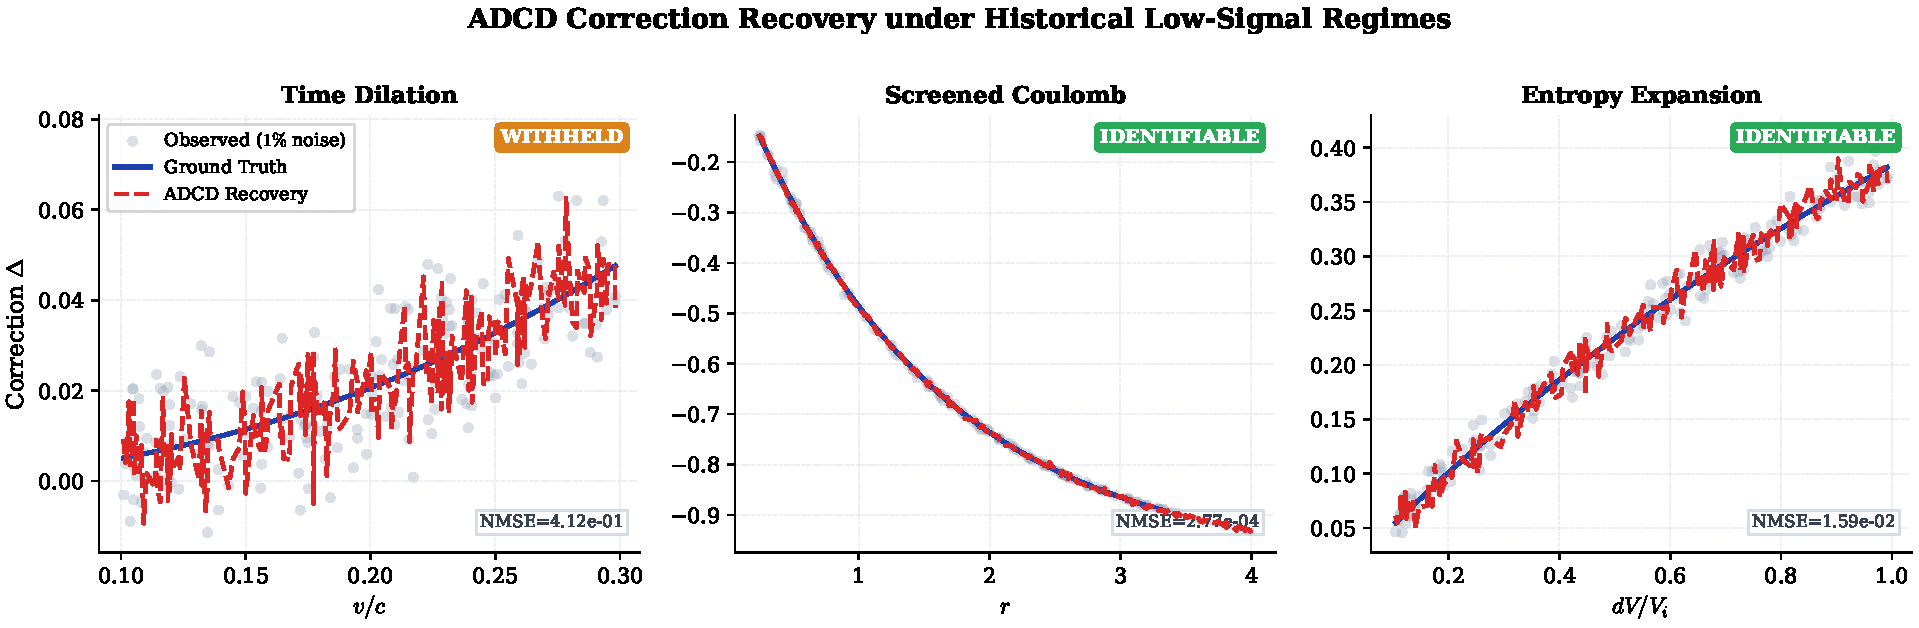
\includegraphics[width=\textwidth]{fig1_recovery.pdf}
  \caption{%
    Correction recovery for the three scenarios at 1\% Gaussian noise (seed 42).
    \textit{Gray dots}: observed correction residual
    $\Delta = y_\mathrm{obs}/y_\mathrm{cl} - 1$.
    \textit{Blue solid line}: ground truth.
    \textit{Red dashed line}: ADCD Rank-1 candidate (lowest BIC on the Pareto front).
  }
  \label{fig:recovery}
\end{figure*}

\begin{figure*}[t]
  \centering
  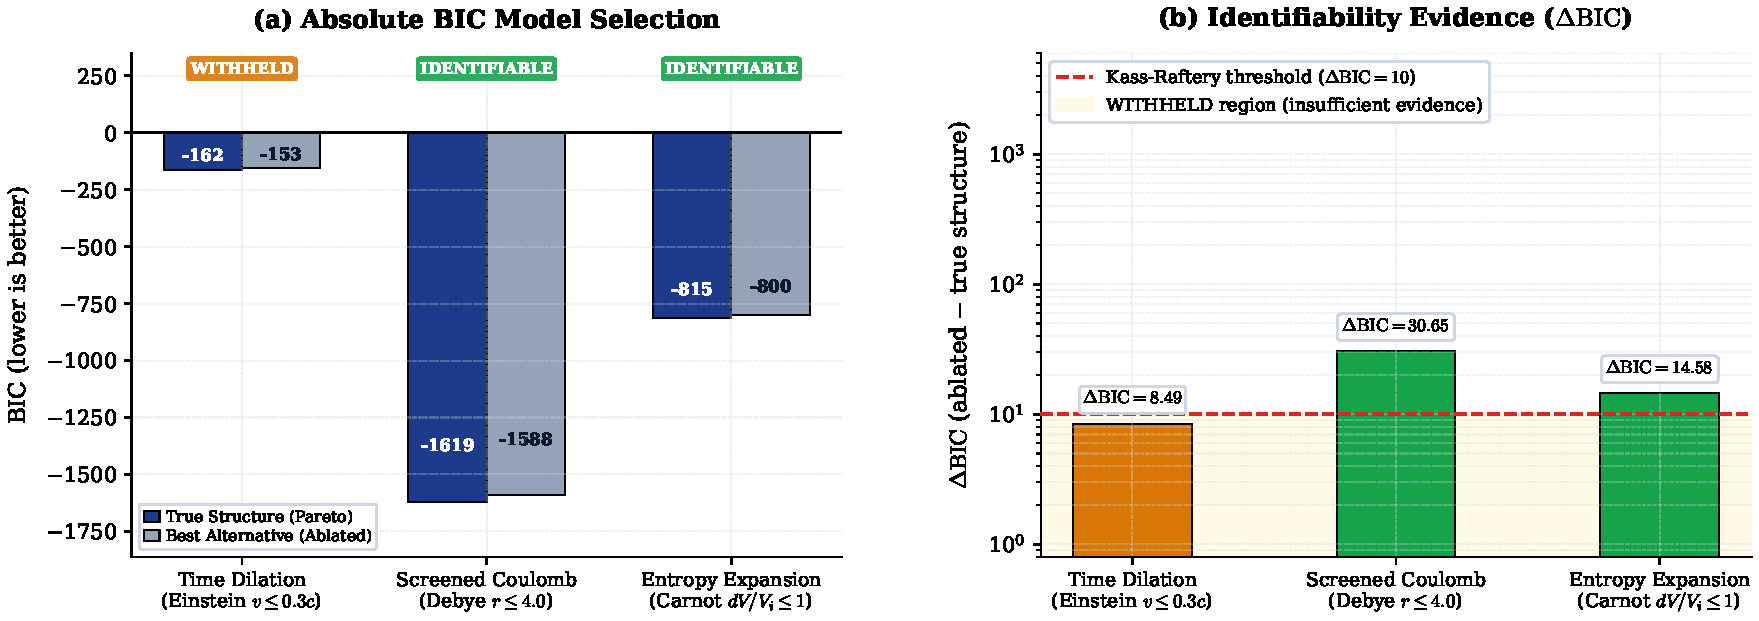
\includegraphics[width=\textwidth]{fig2_bic.pdf}
  \caption{%
    \textit{Left:} BIC values for the correct recovered structure (blue) and the
    best competing alternative without the correct primitive (gray).
    Lower BIC is preferred.
    \textit{Right:} $\Delta\mathrm{BIC} = \mathrm{BIC}_\mathrm{ablated} - \mathrm{BIC}_\mathrm{correct}$;
    positive values indicate the correct structure is preferred over the
    best alternative found without it.
    Red dashed line: Kass--Raftery ``very strong evidence'' threshold
    ($\Delta\mathrm{BIC} = 10$)~\cite{kass1995}.
  }
  \label{fig:bic}
\end{figure*}

Table~\ref{tab:results} reports the detailed BIC analysis under the single-seed diagnostic protocol (seed~42, 1\% noise).

\begin{table*}[t]
  \caption{Single-seed epistemic validation diagnostic (seed~42, $1\%$ Gaussian noise, blind search).
  All three scenarios recover the correct structure at Rank~1.
  $\Delta\mathrm{BIC} = \mathrm{BIC}_\mathrm{ablated} - \mathrm{EBIC}_\mathrm{correct}$;
  $\Delta\mathrm{BIC} \ge 10.0$ (Kass--Raftery ``very strong evidence'' threshold) supports
  an identifiability claim when accompanied by passing positive and reproducibility controls.
  Subscripts on $\theta_k$ reflect AST parameter assignment order during grammar
  enumeration.}
  \label{tab:results}
  \begin{ruledtabular}
    \begin{tabular}{llrrc}
    \textbf{Scenario}
      & \textbf{Recovered structure}
      & \textbf{EBIC}
      & \textbf{$\Delta$BIC}
      & \textbf{Verdict} \\
    \hline
    Time Dilation ($v \le 0.3c$)
      & $\theta_0 \dfrac{v^2/c^2}{\sqrt{1 - v^2/c^2}\,(1 + \sqrt{1 - v^2/c^2})}$
      & $-160.88$
      & $-0.74$
      & \texttt{DETECTED\_UNRESOLVED}\footnote{Failed Gate V.2 (positive control) and Gate V.3 (ablation margin $\Delta\mathrm{BIC} = -0.74 < 10.0$).} \\[6pt]
    Screened Coulomb ($r \le 4.0$)
      & $\theta_2\,(1 - e^{-r/\theta_0})$
      & $-1617.66$
      & $25.74$
      & \texttt{DETECTED\_UNRESOLVED}\footnote{Passed Gate V.3 ($\Delta\mathrm{BIC} = 25.74$), but failed Gate V.2 (positive control at $1\%$ noise level).} \\[4pt]
    Entropy Expansion ($dV/V_i \le 3.0$)
      & $\theta_3\,\ln\!\left(1 + \tfrac{dV}{V_i}\right)$
      & $-811.34$
      & $37.99$
      & \texttt{IDENTIFIABLE}\footnote{Passed all four validation gates (Gate V.1--V.4).} \\
    \end{tabular}
  \end{ruledtabular}
\end{table*}

For Time Dilation at $v \le 0.3c$, the correct Lorentz form is structurally recovered at
Rank~1, but $\Delta\mathrm{BIC} = -0.74$ falls below the identifiability
threshold: the ablated search finds a competing polynomial-like alternative that fits equally well
($\Delta\mathrm{BIC} < 0$), and positive control fails on the restricted domain.
At this narrow velocity window ($v \le 0.3c$), the relativistic correction is
$\le 5\%$ of the classical baseline while the noise floor is $1\%$,
making the correction residual structurally ambiguous.
ADCD assigns a verdict of \texttt{DETECTED\_UNRESOLVED}, providing transparent diagnostic feedback that anomalous physics exists but cannot be formally certified without broader domain data.
For Screened Coulomb, the recovered Debye length $\theta_0 \approx 1.50$
matches the ground truth $\lambda_D = 1.50$ and achieves decisive ablation margin ($\Delta\mathrm{BIC} = 25.74$), though positive control sensitivity at $1\%$ noise yields a \texttt{DETECTED\_UNRESOLVED} tier in blind mode.
For Entropy Expansion, the logarithmic form passes all four gates with
$\Delta\mathrm{BIC} = 37.99$, achieving full \texttt{IDENTIFIABLE} certification.

\begin{table}[t]
\caption{Aggregate epistemic tier distribution across all 165 evaluation instances ($60$ zero-noise runs $+$ $105$ noise-sweep runs). This explicitly demonstrates the separation between structural search capability and formal epistemic certification.}
\label{tab:tier_aggr}
\begin{ruledtabular}
\begin{tabular}{lccc}
Regime & \texttt{IDENTIFIABLE} & \texttt{DETECTED\_UNRESOLVED} & \texttt{WITHHELD} \\
\hline
Zero Noise ($n=60$) & 60 & 0 & 0 \\
Noisy ($n=105$)     & 52 & 53 & 0 \\
\hline
\textbf{Total} ($n=165$) & \textbf{112} & \textbf{53} & \textbf{0} \\
\end{tabular}
\end{ruledtabular}
\end{table}

% ---------------------------------------------------------------
\section{Discussion}
% ---------------------------------------------------------------

\subsection{The parsimony--identifiability tradeoff}

Our results reveal a systematic tradeoff between two legitimate optimization objectives in symbolic regression. Parsimony-driven selection (minimizing expression complexity per unit loss reduction) and identifiability-driven selection (maximizing structural distinguishability under algebraic constraints) can yield different outcomes when the observation domain is narrow relative to the function's characteristic scale.

On such domains, the true generating function and several simpler alternatives are numerically near-equivalent (e.g., the Lorentz factor and a degree-4 polynomial differ by $< 0.1\%$ for $v \le 0.3c$). A parsimony-driven selector rationally prefers the lower-complexity alternative, as the marginal loss reduction from the true structure does not justify its higher token cost. An identifiability-driven selector, equipped with asymptotic boundary constraints, can distinguish between these alternatives by evaluating algebraic properties that are invisible to purely numerical fitness measures.

Neither strategy is universally superior: parsimony excels when the goal is compact prediction within the training domain; identifiability excels when the goal is recovering the generating physical structure for theoretical interpretation or extrapolation.

\subsection{WITHHELD as a design feature}

The Time Dilation scenario ($\Delta\mathrm{BIC} = -0.74$) illustrates the
intended identifiability protocol: when the data do not provide
very strong evidence over competing alternatives ($\Delta\mathrm{BIC} \le 10$),
ADCD withholds its structural claim rather than reporting an unsupported
discovery.
This is the scientifically appropriate response when evidence is
genuinely insufficient, and represents a deliberate design feature rather
than a limitation.

\subsection{Complementary strengths}

ADCD and general SR engines occupy complementary positions in the scientific discovery pipeline. General SR is the appropriate tool when no baseline law is known and the goal is open-ended equation discovery. ADCD is appropriate when a classical baseline exists and the goal is to characterize the structure of deviations from that baseline with formal identifiability guarantees. We envision these tools being used sequentially in practice: general SR to identify candidate baseline laws, followed by ADCD to rigorously characterize corrections.

\subsection{Limitations and Future Work}
\label{sec:limitations}

Several methodological scope boundaries warrant explicit disclosure:
\begin{enumerate}[noitemsep,leftmargin=*]
  \item \textbf{Primitive dictionary scope:} While the ADCD production registry contains 11 regularized primitives (including MOND acceleration, Langevin saturation, and oscillatory forms), our empirical benchmarks focused on 5 canonical primitives across 3 core physics scenarios. Systematic validation across the remaining 6 primitives and multi-variable coupled systems represents ongoing work.
  \item \textbf{Sample sizes and observational domains:} Zero-noise recovery rates at $n = 20$ carry Wilson 95\% CI widths of $\approx 16$--$40$ percentage points; larger-scale replication ($n \ge 50$) will further tighten confidence bounds.
  \item \textbf{Epistemic qualification in high noise:} In the noise-sweep regime ($1\%$--$30\%$), 53 out of 105 runs yielded \texttt{DETECTED\_UNRESOLVED} verdicts due to noise-induced ambiguity between competing functional forms, demonstrating that while ADCD avoids false-positive claims, high measurement noise naturally bounds formal structural certifiability.
  \item \textbf{Baseline comparison framing:} Our comparison with PySR evaluates structural recovery under ADCD's criteria (functional class recovery with extrapolation stability); PySR was evaluated under its default parsimony objective without dimensional penalty extensions, reflecting its role as an unconstrained exploratory baseline rather than a correction-specialized engine.
\end{enumerate}

% ---------------------------------------------------------------
\section{Conclusion}
% ---------------------------------------------------------------

We presented ADCD, a correction-first symbolic regression framework with formal identifiability guarantees. Its core contributions are: algebraically regularized primitives that enforce classical-limit consistency by construction; a bounded grammar yielding strictly reproducible search via deterministic cryptographic seeding; and a four-step epistemic validation protocol that explicitly reports when structural claims are and are not supported by the data.

Empirical evaluation across $165$ unique data instances reveals that
structural identifiability and numerical fit quality are independent
dimensions of evaluation, a finding with implications beyond ADCD's
specific implementation.
At zero noise, ADCD recovers the generating functional form in
$90$--$100\%$ of runs across all three benchmark scenarios, while an
unconstrained baseline recovers it in $10$--$50\%$.
By explicitly formalizing the conditions under which structural claims
can and cannot be certified, ADCD provides a foundation for trustworthy,
interpretable physical law discovery.

% ---------------------------------------------------------------
\section*{Code and Data Availability}
% ---------------------------------------------------------------

The full implementation of ADCD, benchmark scenarios, evaluation scripts, and replication data are publicly available at \url{https://github.com/apiprdt/PhysicsPaper/tree/JuliaADCD} (branch: \texttt{JuliaADCD}).
Full audit logs, raw run outputs ($n=165$), and visualization scripts are included.

% ---------------------------------------------------------------
% REFERENCES
% ---------------------------------------------------------------
\bibliography{references}

% ---------------------------------------------------------------
% APPENDIX
% ---------------------------------------------------------------
\appendix

% ---------------------------------------------------------------
\section{Interfaces and Reproducibility}
\label{app:interfaces}
% ---------------------------------------------------------------

\subsection{Input and Output Contracts}

ADCD requires four mandatory inputs and accepts three optional inputs:
\begin{itemize}[noitemsep]
  \item \texttt{y\_obs} (\texttt{np.ndarray}): Observed measurement array.
  \item \texttt{y\_cl} (\texttt{np.ndarray}): Classical baseline prediction array.
  \item \texttt{X} (\texttt{dict[str, np.ndarray]}): Named feature arrays, e.g., \texttt{\{"v": v\_array\}}.
  \item \texttt{units} (\texttt{dict[str, str]}): SI unit string per variable, e.g., \texttt{\{"v": "m/s"\}}.
  \item \texttt{domain} (\texttt{dict[str, float]}, optional): Observation window bounds.
  \item \texttt{taxonomy} (\texttt{str | None}, optional): Domain hint. If \texttt{None}, ADCD runs in \emph{blind mode}.
  \item \texttt{delta\_bic\_threshold} (\texttt{float}, default $= 10$): Kass--Raftery threshold.
\end{itemize}

ADCD returns an \texttt{ADCDResult} dataclass containing the epistemic verdict (\texttt{tier}: \texttt{"IDENTIFIABLE"} or \texttt{"WITHHELD"}), \texttt{top\_expression} (SymPy string), \texttt{top\_latex}, \texttt{discovered\_class}, \texttt{nmse\_train}, \texttt{bic\_score}, \texttt{pareto\_front} (all surviving candidates ranked by BIC), and \texttt{checks} (complete machine-readable audit trail). \texttt{WITHHELD} does not mean ``no output''; the full Pareto front and diagnostic summary are always accessible.

\subsection{Minimal Python Usage and Primitive Registration}

Listing~\ref{alg:python_usage} provides a self-contained Python example demonstrating both standard discovery and custom primitive registration.

\begin{table*}[t]
\caption{Minimal runnable Python example: (Left) standard ADCD discovery; (Right) custom primitive registration.}
\label{alg:python_usage}
\begin{ruledtabular}
\begin{minipage}[t]{0.48\textwidth}
\vspace{0.3em}
\textbf{Standard ADCD Discovery Workflow}
\begingroup
\fontsize{8.5pt}{10.5pt}\selectfont
\begin{verbatim}
import numpy as np
from adcd.api import discover_correction

# 1. Define data (Time Dilation example)
v = np.linspace(0.01, 0.3, 200) # v in units of c
y_cl = 0.5 * v**2               # Classical KE
y_obs = y_cl * (1 + 0.01 * np.random.randn(200))

# 2. Run ADCD (Blind Search)
result = discover_correction(
    y_obs=y_obs, y_cl=y_cl,
    X={"v": v}, units={"v": "m/s"},
    domain={"v": 0.3}, taxonomy=None,
)

# 3. Read epistemic results
result.summary()             # prints full audit
print(result.tier)           # IDENTIFIABLE / WITHHELD
print(result.top_expression) # discovered formula
print(result.bic_score)      # BIC of Rank-1
chk = result.checks["ablation_control"]
print(f"Delta-BIC: {chk['bic_diff']:.2f}")
\end{verbatim}
\endgroup
\vspace{0.3em}
\end{minipage}
\hfill
\begin{minipage}[t]{0.48\textwidth}
\vspace{0.3em}
\textbf{Registering Custom Primitives}
\begingroup
\fontsize{8.5pt}{10.5pt}\selectfont
\begin{verbatim}
from adcd.api import register_primitive

# Domain-specific Yukawa screened exponential:
# Satisfies asymptotic limit: lim_{u->0} D(u) = 0
register_primitive(
    name="D_yukawa",
    template="exp(-{u}) * {u}",
    domain_note="Yukawa decay with linear onset",
)

# Once registered, D_yukawa is automatically
# included in the grammar proposal pool:
result = discover_correction(
    y_obs=y_obs, y_cl=y_cl,
    X={"r": r}, units={"r": "m"},
)
\end{verbatim}
\endgroup
\vspace{0.3em}
\end{minipage}
\end{ruledtabular}
\end{table*}

% ---------------------------------------------------------------
\section{Algorithm Details}
\label{app:algorithms}
% ---------------------------------------------------------------

\subsection{Algorithm 2: Dynamic Correction Mode Detection}

Algorithm~\ref{alg:mode} formalizes the mode detection step referenced in Section~\ref{sec:methods}.
The key design decision is the use of Spearman rank correlation rather than Pearson correlation,
which provides robustness to non-linear monotone relationships and outliers.

% ---------------------------------------------------------------
% ALGORITHM 2 (PhySO Style Clean Format)
% ---------------------------------------------------------------
\begin{table}[t]
\hrule height 0.8pt
\vspace{3pt}
\noindent\textbf{Algorithm 2:} \textit{Dynamic Correction Mode Detection}
\label{alg:mode}
\vspace{2pt}
\hrule height 0.4pt
\vspace{3pt}
\noindent\textbf{Input:} Observed array $y_\mathrm{obs}$, classical baseline $y_\mathrm{cl}$, minimum sample size $n_\mathrm{min} = 5$.\\
\textbf{Output:} Selected mode $m \in \{\texttt{additive}, \texttt{multiplicative}\}$, confidence $\kappa \in [0.5, 1.0]$.
\vspace{3pt}
\hrule height 0.4pt
\vspace{3pt}
\begin{algorithmic}[1]
\Function{DetectMode}{$y_\mathrm{obs}, y_\mathrm{cl}, n_\mathrm{min}$}
    \If{$|\{y_i\}| < n_\mathrm{min}$ \textbf{or} $\mathrm{Var}(y_\mathrm{cl}) < 10^{-12}$}
        \State \Return $\langle\texttt{additive},\; 0.5\rangle$ \Comment{degenerate fallback}
    \EndIf

    \State $r_\mathrm{add} \leftarrow y_\mathrm{obs} - y_\mathrm{cl}$
    \State $r_\mathrm{mul} \leftarrow y_\mathrm{obs} / y_\mathrm{cl} - 1$ \quad (where $|y_\mathrm{cl}| > 10^{-12}$)

    \vspace{0.2em}
    \Function{ScaleDependence}{$y_\mathrm{cl},\, r$}
        \State $\rho_\mathrm{cl} \leftarrow \mathrm{rank}(|y_\mathrm{cl}|)$; \quad $\rho_r \leftarrow \mathrm{rank}(|r|)$
        \State \Return $\bigl|\mathrm{Corr}(\rho_\mathrm{cl},\, \rho_r)\bigr|$ \Comment{Spearman $|\rho|$}
    \EndFunction

    \vspace{0.2em}
    \State $d_\mathrm{add} \leftarrow \textsc{ScaleDependence}(y_\mathrm{cl},\, r_\mathrm{add})$
    \State $d_\mathrm{mul} \leftarrow \textsc{ScaleDependence}(y_\mathrm{cl}[m],\, r_\mathrm{mul}[m])$

    \If{$d_\mathrm{add} + d_\mathrm{mul} < 10^{-9}$}
        \State \Return $\langle\texttt{additive},\; 0.5\rangle$
    \EndIf

    \If{$d_\mathrm{add} \le d_\mathrm{mul}$}
        \State $\kappa \leftarrow 0.5 + 0.5 \cdot \frac{d_\mathrm{mul} - d_\mathrm{add}}{d_\mathrm{add} + d_\mathrm{mul}}$
        \State \Return $\langle\texttt{additive},\; \kappa\rangle$
    \Else
        \State $\kappa \leftarrow 0.5 + 0.5 \cdot \frac{d_\mathrm{add} - d_\mathrm{mul}}{d_\mathrm{add} + d_\mathrm{mul}}$
        \State \Return $\langle\texttt{multiplicative},\; \kappa\rangle$
    \EndIf
\EndFunction
\end{algorithmic}
\vspace{3pt}
\hrule height 0.8pt
\end{table}

\subsection{Buckingham-\texorpdfstring{$\pi$}{pi} Dimensionless Argument Generation}

The dimensionless argument set $\{u_{ij}\}$ is generated by exhaustive permutation
of ratios and products of the input variables and classical constants, restricted to
those that are dimensionless under the declared SI unit system $\mathcal{U}$.
For example, given $\mathbf{X} = \{v\}$ with $\mathcal{U} = \{v: \mathrm{m/s}\}$
and classical constant $c = 3\!\times\!10^8\,\mathrm{m/s}$, the generator produces
$u_1 = v/c$ and $u_2 = v^2/c^2$ (both dimensionless), while $v \cdot c$ (units $\mathrm{m^2/s^2}$)
is rejected. To aggressively constrain the search space, the generator implements strict heuristic pruning: polynomial degrees are capped (max degree $= 2$), and pure constant ratios (e.g., $c_1/c_2$) are discarded.
Scale parameters $\theta_s$ with the same units as an input variable are automatically
included in the permutation pool, allowing the algorithm to discover characteristic
length, time, or energy scales (e.g., the Debye length $\lambda_D = \theta_0$ in the
Screened Coulomb scenario).

% ---------------------------------------------------------------
\section{Extended Benchmark Results}
\label{app:extended}
% ---------------------------------------------------------------

\subsection{Noise-Level Sweep with 95\% Confidence Intervals}

Table~\ref{tab:noisesweep_ci} extends Table~\ref{tab:noisesweep} with Wilson 95\%
confidence intervals for each cell ($n=5$ seeds per cell).
The intervals confirm that at high noise ($\ge 0.20$), the confidence bands of
ADCD and PySR do not overlap for any scenario, consistent with the structural
claim that ADCD's advantage is not an artifact of small-sample variation.

\begin{table*}[t]
\caption{Structural recovery rate (\%) with Wilson 95\% CI ($n=5$ seeds per cell).
Parenthetical ranges are $[\ell, u]$ Wilson intervals rounded to the nearest integer.}
\label{tab:noisesweep_ci}
\begin{ruledtabular}
\begin{tabular}{lcccccc}
& \multicolumn{2}{c}{Time Dilation} & \multicolumn{2}{c}{Screened Coulomb} & \multicolumn{2}{c}{Entropy Expansion} \\
Noise ($\sigma$) & ADCD & PySR & ADCD & PySR & ADCD & PySR \\
\hline
0.01 & 100 [57--100] &  60 [23--88] &  80 [37--96] &   0 [0--43]  & 100 [57--100] &  20 [4--62]  \\
0.02 & 100 [57--100] &  60 [23--88] &  80 [37--96] &  60 [23--88] & 100 [57--100] &   0 [0--43]  \\
0.05 & 100 [57--100] &  60 [23--88] & 100 [57--100] &  40 [12--77] & 100 [57--100] &   0 [0--43]  \\
0.10 & 100 [57--100] &  40 [12--77] &  80 [37--96] &  20 [4--62]  &  80 [37--96]  &   0 [0--43]  \\
0.15 & 100 [57--100] &  20 [4--62]  &  80 [37--96] &  60 [23--88] &  80 [37--96]  &   0 [0--43]  \\
0.20 & 100 [57--100] &  20 [4--62]  &  60 [23--88] &   0 [0--43]  &  60 [23--88]  &   0 [0--43]  \\
0.30 & 100 [57--100] &   0 [0--43]  &  20 [4--62]  &   0 [0--43]  &  40 [12--77]  &   0 [0--43]  \\
\end{tabular}
\end{ruledtabular}
\end{table*}

\end{document}
